% Created 2022-03-29 Tue 11:59
% Intended LaTeX compiler: pdflatex
\documentclass{beamer}
\usetheme{default}
\date{\today}
\title{}
\hypersetup{
 pdfauthor={},
 pdftitle={},
 pdfkeywords={},
 pdfsubject={},
 pdfcreator={Emacs 27.2 (Org mode 9.5.2)}, 
 pdflang={English}}
\begin{document}

\begin{frame}{Outline}
\tableofcontents
\end{frame}

\chapter{Intro}
\label{sec:org30d38ea}
\begin{frame}[label={sec:orgece807b},fragile]{Goal}
 \begin{enumerate}
\item \alert{semantic  analysis}, as far as 
\begin{itemize}
\item \alert{typing} is concerned (``static semantics'')
\item other coditions (no duplicate declaration etc)
\end{itemize}

\item \alert{code generation} for \texttt{compila22} (ish) programs
\end{enumerate}
\end{frame}






\begin{frame}[label={sec:org8f7d745}]{Last time (O1)}
\begin{block}{Syntactic analysis}
\begin{itemize}
\item lexer (scanner)
\item parser
\item abstract syntax tree
\end{itemize}
\end{block}



\alert{this time}: continue with your previous deliv. (and repos)
\end{frame}



\begin{frame}[label={sec:org4561e89}]{Learning outcome}
\begin{itemize}
\item understand type checking, implementing a simple variant
\end{itemize}


\begin{itemize}
\item understand (simple form of) bytecode and how to generate it from ``source
code'' (as AST)

\item extend an existing compiler code base with new functionality
\end{itemize}
\end{frame}


\chapter{Semantic analysis}
\label{sec:org0db736d}
\begin{frame}[label={sec:orgd317740}]{Semantic analysis \& type checking}
\begin{itemize}
\item parser / context-free  grammars 
\begin{itemize}
\item not powerful enough
\item cannot check all (static) properties of a language spec
\end{itemize}

\item => extend the front-end by a type checker

\begin{itemize}
\item use the AST classes of last time
\item add type checking code
\item allowed to make \alert{changes} or adaptations if advantagous.
\end{itemize}
\end{itemize}
\end{frame}


\begin{frame}[label={sec:orgac88ad2}]{Another glance at compila22}
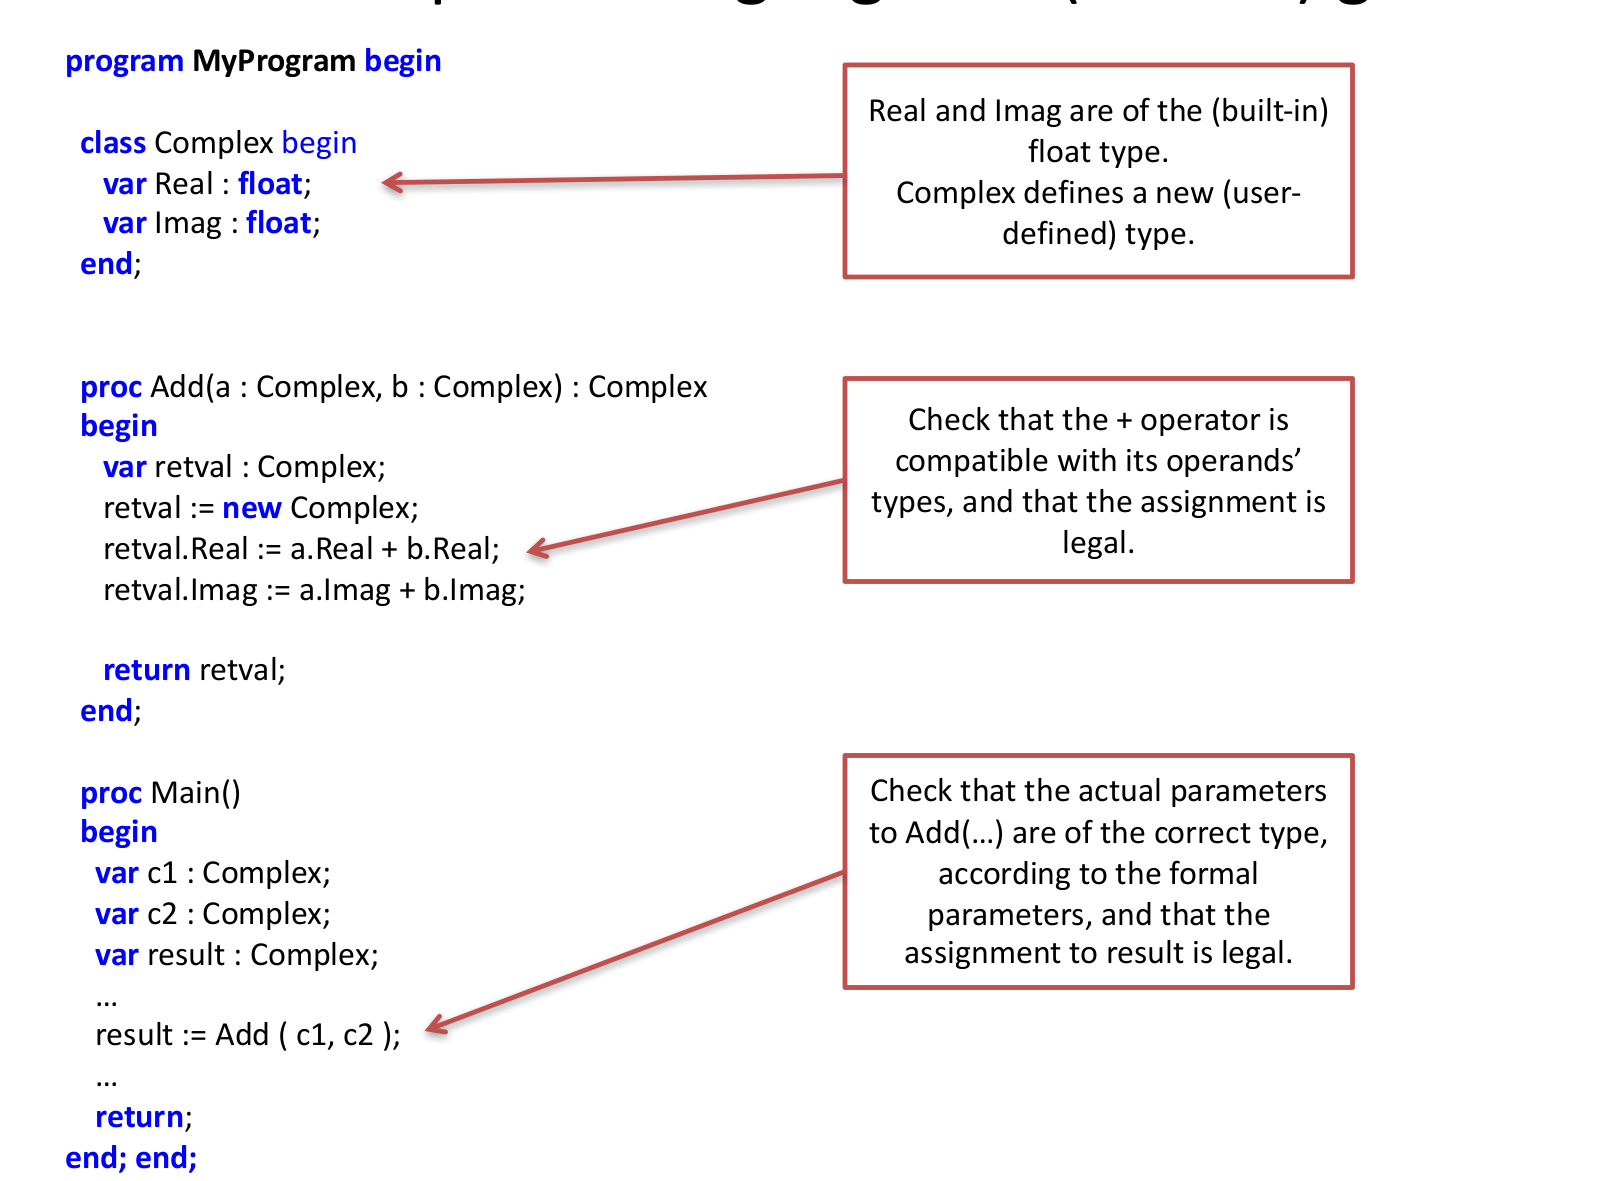
\includegraphics[width=\textwidth]{figures/snaps/compilaexample-checking}


NB: 2022: structs, not classes 
\end{frame}


\begin{frame}[label={sec:org0fc0cf7},fragile,plain]{Type checking for conditionals}
 \begin{itemize}
\item as ``inspiration'', details may vary
\end{itemize}


\lstset{language=java,label= ,caption= ,captionpos=b,numbers=none}
\begin{lstlisting}
  class IfStatement extends Statement {
  ...
    public void typeCheck(){
      String condType = condition.get.Type ();
      if (condType != "bool") {  
	 throw new TypeException("condition in an if 
	   statement must be of type bool")
      }
}
\end{lstlisting}
\end{frame}


\begin{frame}[label={sec:orgd6f2d3b},fragile,plain]{Type checking: assignments}
 \lstset{language=java,label= ,caption= ,captionpos=b,numbers=none}
\begin{lstlisting}
class Assignment extends Statement {
...
  public void typeCheck() {
    String varType = var.getType();
    String expType = exp.getType();
    if (varType != expType &&
       !isAssigmentCompatible(varType,expType){
		 throw new TypeException("Cannot assign " + vartpe + 
		 " from " + expType);
  }
}

\end{lstlisting}
\end{frame}



\chapter{Code generation}
\label{sec:orgced0969}
\begin{frame}[label={sec:org9eec11f},fragile]{Code generation}
 \begin{itemize}
\item byte code API and operations are described in the document ``Interpreter
and bytecode for INF5110''

\item \alert{Task:} add bytecode generation methods to your AST classes
for instance
\end{itemize}

\begin{verbatim}
Ast.Node.GenerateCode(...)
\end{verbatim}
\begin{itemize}
\item again: if adaptations of the AST are called for or useful, go for it\ldots{}

\item some people did \alert{visitors} for ast-printing, one can also (re-)use the visitor pattern
\end{itemize}
\end{frame}

\begin{frame}[label={sec:orgf0194ee},fragile]{Code generation: limitations}
 \begin{itemize}
\item interpreter and byte code library somewhat \alert{limited}
\begin{itemize}
\item cannot express full compila 22
\item no block structure
\item no reference types
\end{itemize}
\end{itemize}


\begin{itemize}
\item your delivery should support generating correct bytecode
for the \texttt{compila} 22 source code file \texttt{runme.cmp}
\end{itemize}
\end{frame}



\begin{frame}[label={sec:orgf693d3c},fragile,plain]{Code generation: creating a procedure}
 \lstset{language=java,label= ,caption= ,captionpos=b,numbers=none}
\begin{lstlisting}
CodeFile codeFile = new CodeFile();
// add the procedure by name first
codeFile.addProcedure("Main")
// then define it
CodeProcedure main = new 
   CodeProcedure("Main", VoidType,TYPE, codeFile);
main.addInstruction( new RETURN());
//then update it in the code file
codeFile.updateProcedure(main);
\end{lstlisting}
\end{frame}

\begin{frame}[label={sec:org6b1c101}]{Code generation: assignment}
\begin{center}
 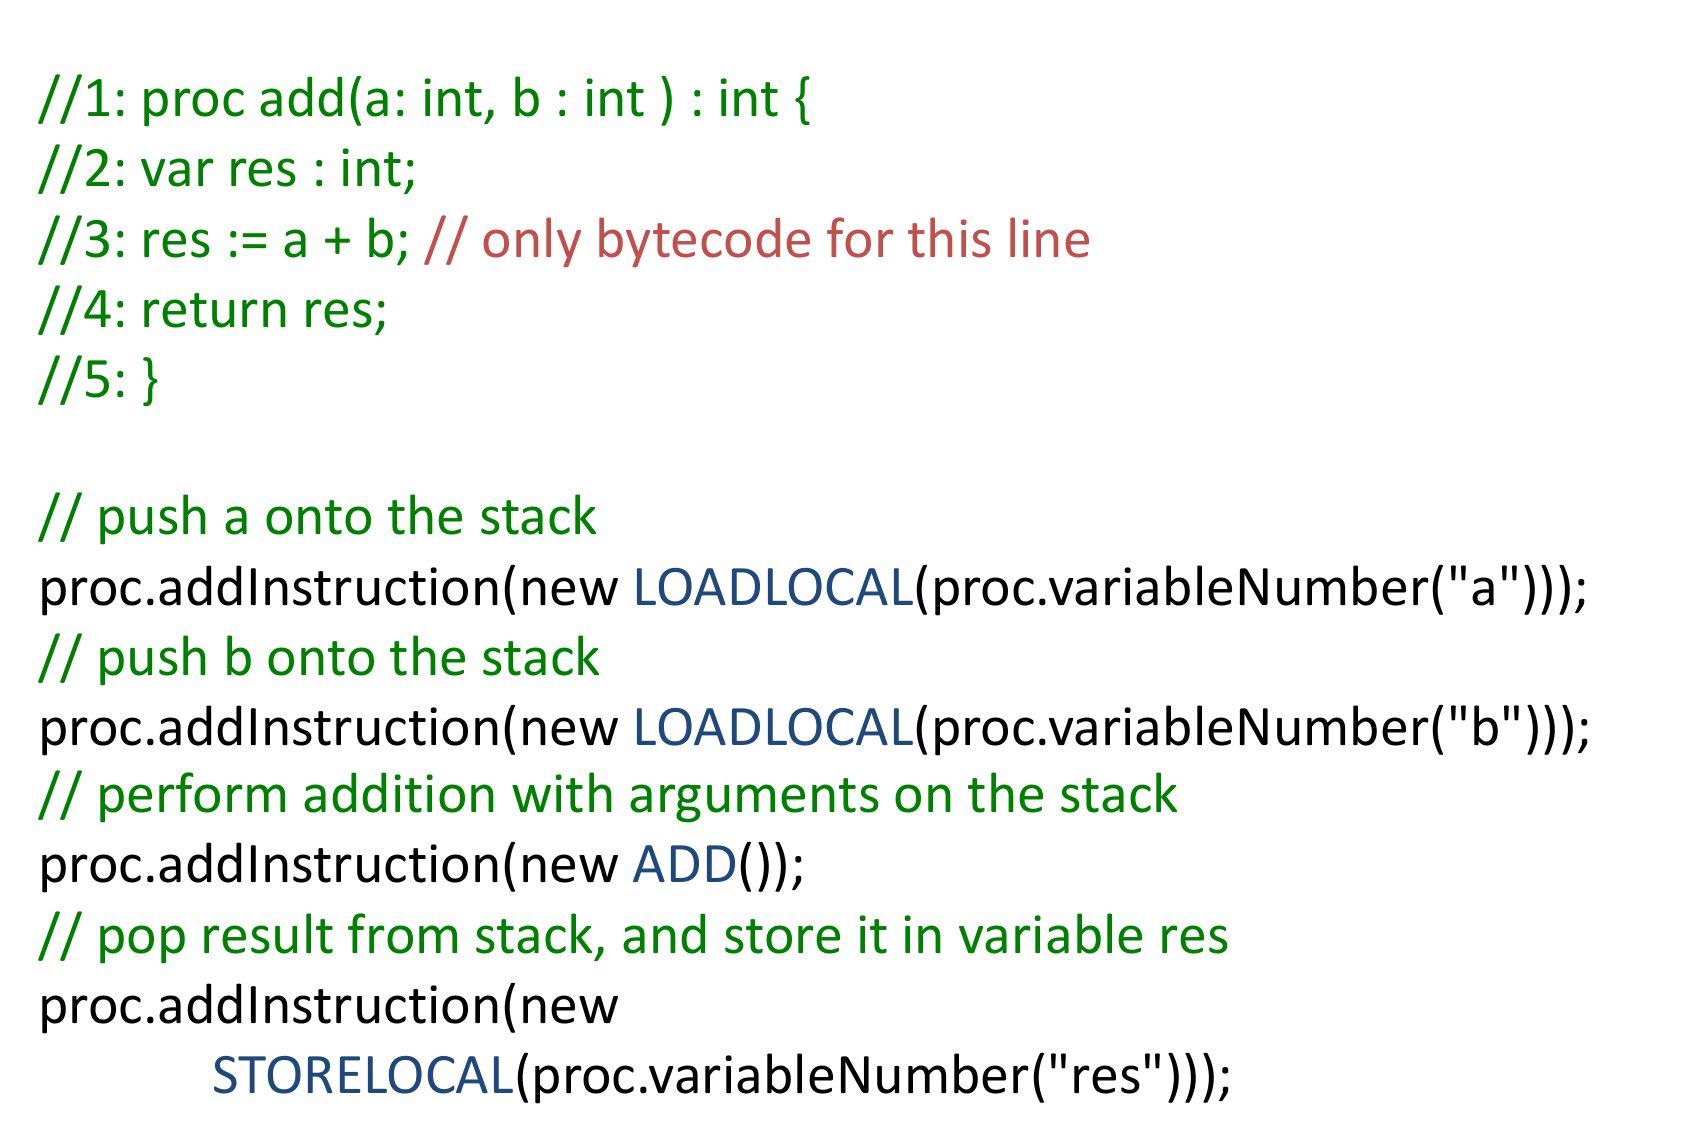
\includegraphics[width=0.76\textwidth]{figures/snaps/codegen-assignment}
\end{center}
\end{frame}


\chapter{Testing}
\label{sec:org5bb3ec1}
\begin{frame}[label={sec:org5fd7afd},fragile]{Testing}
 \begin{itemize}
\item bunch of test files, for testing the \emph{type checker}
\item preferable: make \texttt{ant test} workable

\item test files inside \texttt{./tests/semanticanalysis/errors/} (and with \texttt{fail} in
the filename) contain a syntactically correct but erronous program
(erroneous as the type system or generally the semantic phase is
concerned)

\item => compiler returns error code 2 for semantic failure
\end{itemize}
\end{frame}



\chapter{Starting point and hand in}
\label{sec:org7661899}
\begin{frame}[label={sec:orgcf88f46}]{Provided source code (patch)}
\url{https://github.uio.no/msteffen/compila}

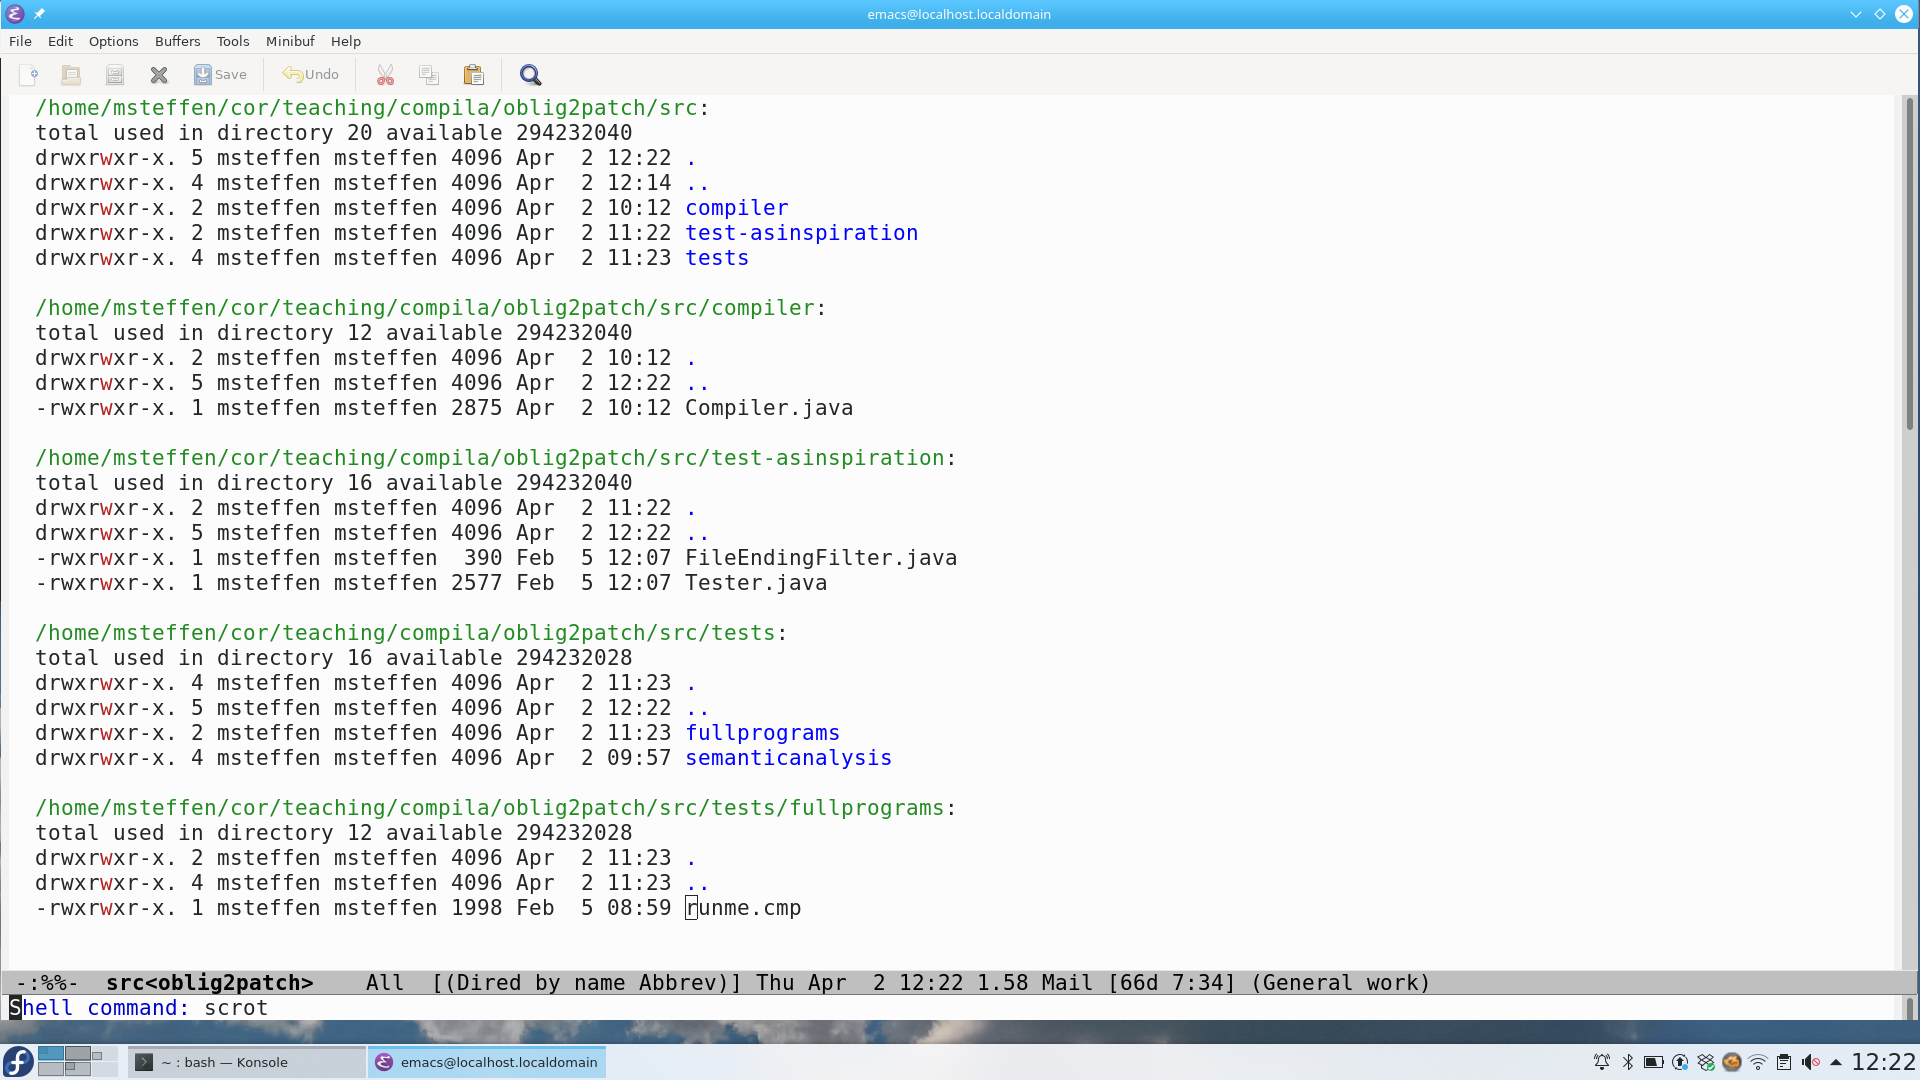
\includegraphics[width=0.96\textwidth]{figures/snaps/directorystructure-src}

Tests: already included in the oblig1 checkout, so left out in the zip-patch
this year.
\end{frame}

\begin{frame}[label={sec:orgf53f651}]{Provided documentation (patch)}

\begin{center}
 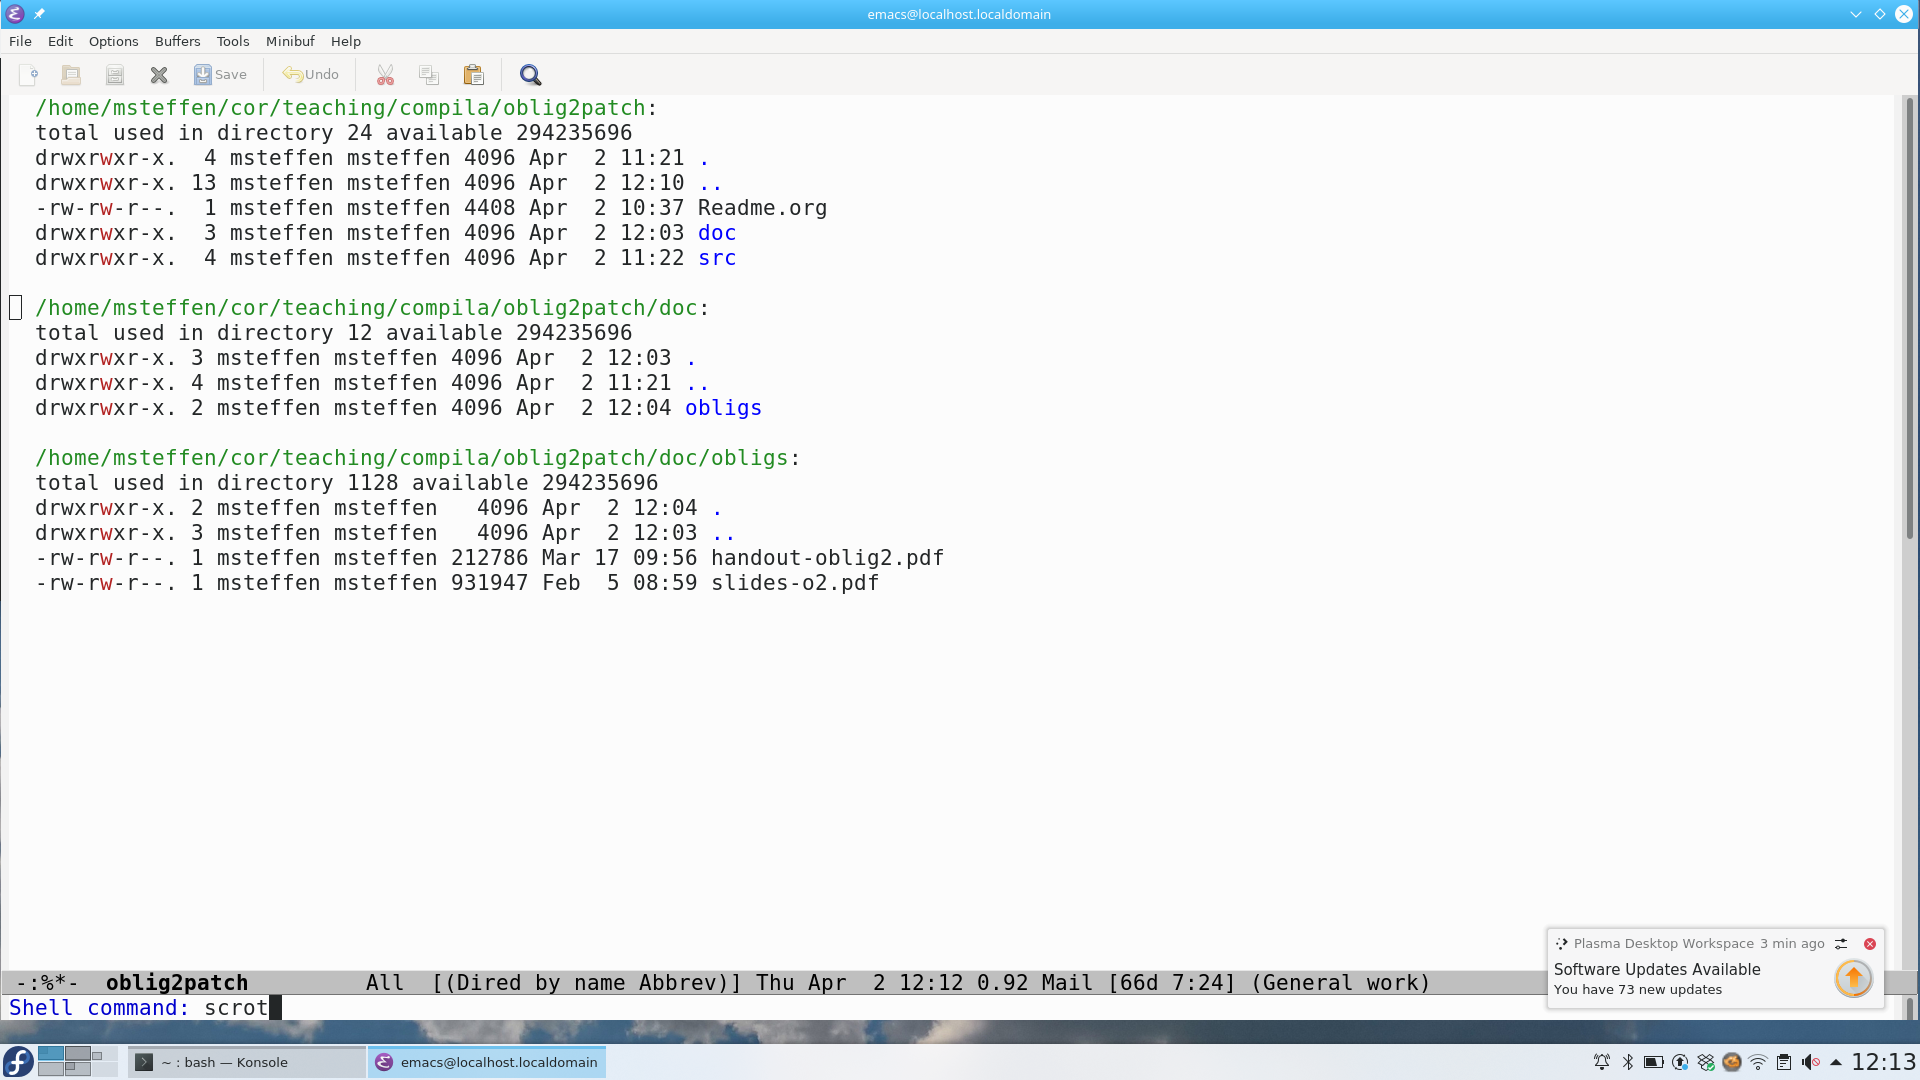
\includegraphics[width=0.75\textwidth]{figures/snaps/directorystructure-doc}
\end{center}
\end{frame}



\begin{frame}[label={sec:org719f5d4},fragile]{Relevant directories}
 \begin{itemize}
\item Java

\begin{itemize}
\item \texttt{compiler}: updated compiler class (patch)
\item \texttt{test}:   some code for performing tests (patch)
\item \texttt{bytecode}: classes for constructing bytecode (already there)
\item \texttt{runtime}: rte for executing the byte code (already there)
\end{itemize}

\item Compila

\begin{itemize}
\item \texttt{tests}: some test files (including \texttt{runme.cmp})
\end{itemize}
\end{itemize}
\end{frame}



\begin{frame}[label={sec:org3812f8a},fragile]{Deadline}
 \begin{alertblock}{Deadline}
(9 May 2022)
\end{alertblock}


Note: end of semester, and I need to report the ones passing the oblig some
time before the exam.


\begin{block}{delivs}
\begin{itemize}
\item working type checker
\item code generator (test with \texttt{runme.cmp})
\item report (including your name(s) etc.

\begin{itemize}
\item discussion of your solution, choices you made, assumptions you rely on

\item printout of a test run (can be also checked in into the repos, but it 
needs to be mentioned where it is)
\item printout of the bytecode from \texttt{runme.cmp} (with a target like \texttt{ant
    list-runme})

\item solution must ``build'' and be ``testable'' (typically via \texttt{ant})
\end{itemize}
\end{itemize}
\end{block}
\end{frame}
\end{document}